\documentclass[12pt,a4paper,titlepage]{article}
\usepackage[utf8]{inputenc}
\usepackage{polski}
\usepackage{listings}
\usepackage{graphicx}
\usepackage{xcolor}
\usepackage{minted}
\makeatletter
\newcommand{\linia}{\rule{\linewidth}{0.4mm}}
\renewcommand{\maketitle}{\begin{titlepage}
    \vspace*{1cm}
    \begin{center}\small
    Politechnika Wrocławska\\
    Wydział Elektroniki\\
    Urządzenia cyfrowe i systemy wbudowane 1
    \end{center}
    \vspace{3cm}
    \noindent\linia
    \begin{center}
      \LARGE \textsc{\@title}
         \end{center}
     \linia
    \vspace{0.5cm}
    \begin{flushright}
    \begin{minipage}{7cm}
    \textit{\small Autor:}\\
    \normalsize \textsc{\@author} \par
    \end{minipage}
    \vspace{5cm}

     {\small Wtorek, 7\textsuperscript{30}-10\textsuperscript{15} TP}\\
        Dr inż. Dariusz Caban
     \end{flushright}
    \vspace*{\stretch{6}}
    \begin{center}
    \@date
    \end{center}
  \end{titlepage}%
}
\makeatother
\author{Justyna Skalska, 225942\\
        Piotr Pawelski, 218370}
\title{Sprawozdanie nr 3\\
\large(Zamek szyfrowy)}

\begin{document}
\maketitle

\section{Wstęp}
Celem laboratorium było zaprojektowanie schematu automatu otwierającego zamek szyfrowy. Hasło składało się z 4 cyfr: 3142. Przyciski znajdujące się na płytce odpowiadały poszczególnym cyfrom od 1 do 4. Dodatkowy przycisk odpowiadał za reset stanu automatu. Zaświecenie się diody oznaczało poprawne otwarcie zamka szyfrowego.\\\\
Programem wykorzystanym do wykonania zadania jest ISE Design Suite.

\section{Przebieg zajęć}
Zajęcia rozpoczęliśmy od wymyślenia naszego szyfru. Później zajęliśmy się projektowaniem stanów automatu oraz przejść pomiędzy nimi. Do stworzenia układu wykorzystaliśmy przerzutniki T.
\begin{figure}[H]
\centering
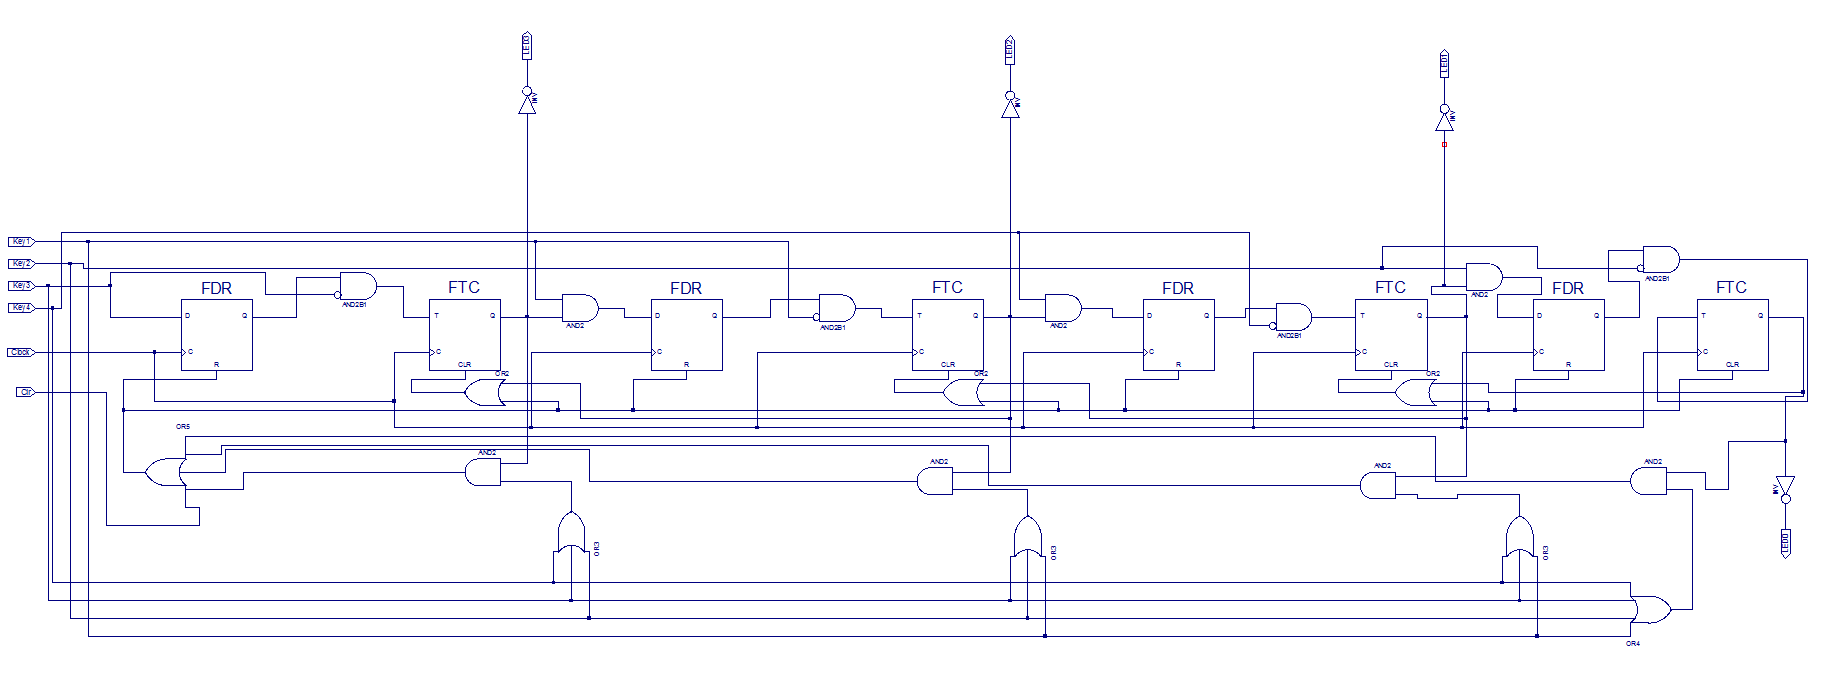
\includegraphics[angle=90,height=20cm]{schemat.png}
\caption{Schemat układu}
\label{fig:schemat}
\end{figure}

Kolejnym etapem było wygenerowanie pliku VHDL oraz zmodyfikowanie go w taki sposób, aby odpowiadał naszym potrzebom.

\begin{listing}[H]
\caption{Kod VHDL}
\begin{minted}[linenos,breaklines]{vhdl}
LIBRARY ieee;
USE ieee.std_logic_1164.ALL;
USE ieee.numeric_std.ALL;
LIBRARY UNISIM;
USE UNISIM.Vcomponents.ALL;
ENTITY SZYFR_SZYFR_sch_tb IS
END SZYFR_SZYFR_sch_tb;
ARCHITECTURE behavioral OF SZYFR_SZYFR_sch_tb IS 

   COMPONENT SZYFR
   PORT(  Key1  :   IN  STD_LOGIC; 
          Key2  :   IN  STD_LOGIC; 
          Key3  :   IN  STD_LOGIC; 
          Key4  :   IN  STD_LOGIC; 
          Clr   :   IN  STD_LOGIC; 
          Clock :   IN  STD_LOGIC; 
          LED0  :   OUT STD_LOGIC);
   END COMPONENT;

   SIGNAL Key1  :   STD_LOGIC;
   SIGNAL Key2  :   STD_LOGIC;
   SIGNAL Key3  :   STD_LOGIC;
   SIGNAL Key4  :   STD_LOGIC;
   SIGNAL Clr   :   STD_LOGIC;
   SIGNAL Clock :   STD_LOGIC;
   SIGNAL LED0  :   STD_LOGIC;

BEGIN

   UUT: SZYFR PORT MAP(
		Key1 => Key1, 
		Key2 => Key2, 
		Key3 => Key3, 
		Key4 => Key4, 
		Clr => Clr, 
		Clock => Clock, 
		LED0 => LED0
   );
END;
\end{minted}
\end{listing}

\begin{itemize}
    \item \textbf{Key1 -- Key4} to kolejne przyciski odpowiadające cyfrom od 1 do 4
    \item \textbf{Clr} to przycisk odpowiadający za reset układu
    \item \textbf{Clock} to wejście układu odpowiadające za dostarczenie sygnału zegara.
    \item \textbf{LED0} to dioda, której zapalenie się oznacza udane otwarcie zamka
\end{itemize}
Następnym zadaniem, które wykonaliśmy było skompilowanie układu oraz wygenerowanie pliku .jed, który jest używany do programowania mikroprocesorów. Następnie przesłaliśmy nasz program na płytkę, gdzie udało nam się poprawnie wpisać szyfr oraz otworzyć zamek.

\section{Wnioski}
Podczas laboratoriów mogliśmy zapoznać się z podstawami tworzenia automatów przy użyciu programu ISE Design Suite.
\end{document}